\section{Demonstration}
To demonstrate the capabilities of the modified version of DocetOS, we will attempt to simulate a portion of the priority inversion problem faced by the Mars Pathfinder mission \cite{MarsPathfinder}, and show that our program is not only able to replicate the problem, but overcome it.\hfill\newline
To accomplish this, we will consider the following scenario:
\begin{center}
	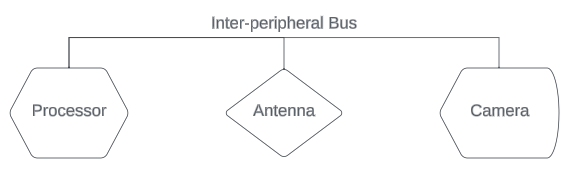
\includegraphics[width=1\textwidth]{bus.png}
\end{center}
We have a simple system with a processor, antenna, and camera. The processor is responsible for sending commands to peripherals, along with a  myriad of other devices it is simultaneously connected to, and hence is running multiple tasks concurrently. The camera is responsible for capturing images to be sent back to earth, which it sends to the antenna. The antenna waits until it has received a specified number of images (in our demonstration, we will use 10), filling its internal buffer, and then sends the images to earth for analysis.\hfill\newline

The challenge with this system, is that the processor, antenna, and camera all share the same bus. So, a mutex is required to protect the bus against being accessed by multiple tasks simultaneously. In the Mars PathFinder mission, it led to the following priority inversion problem when software engineers accidentally did not set the mutex to operate with priority inheritance. Consider 3 tasks of ascending priority:\hfill\newline

\noindent
\textbf{Task A (high priority)} – polls the antenna regularly to verify the internal buffer level. When at capacity, it sends a command to the antenna to send all stored data, emptying the buffer.\hfill\newline

\noindent
\textbf{Task B (Medium priority)} – a miscellaneous task related to other areas of the system which take up processing time.\hfill\newline

\noindent
\textbf{Task C (Low priority)} – Sends an instruction to the camera to take 10 images in succession and send them to the antenna, filling up the antennas buffer.\hfill\newline

\noindent
Without mutex priority inheritance, the combination of the timing of these tasks causes the following to occur: 
\begin{center}
	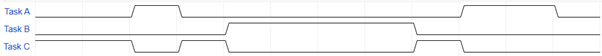
\includegraphics[width=1\textwidth]{inversion.png}
\end{center}
As we can see due to Task B becoming active during the execution of Task C, the completion of Task C and consequently task A is delayed considerably, slowing down the filling of the antenna buffer.  While this is not exactly how the Mars PathFinder priority inversion incident occurred, during the mission this task incident caused the automatic watchdog timer on the craft to trigger, resetting the entire system daily. In our demonstration, turning off mutex priority inheritance causes the same behaviour, slowing down the population of the antenna buffer with data, making the system unsuitable for real-world use.\hfill\newline
To remedy the priority inversion vulnerability, we activate our mutexes priority inheritance functionality, correcting the system to the intended behaviour seen below:
\begin{center}
	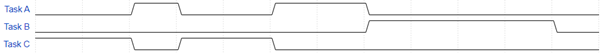
\includegraphics[width=1\textwidth]{noinversion.png}
\end{center}
Instead of Task C being interrupted by Task B, Task C inherits a higher priority due to the mutex priority inheritance, allowing it to run to completion freeing up the shared resource for Task A to complete. Then the miscellaneous Task B can freely run. The corrected behaviour demonstrates the enhanced functionality offered by our modifications. Specifically, we can see:
\begin{itemize}[]
	\item The priority scheduler correctly scheduling higher priority tasks above lower priority tasks.
	\item Task sleeping, as the higher priority task only runs when it polls the antenna state, instead of constantly, avoid system deadlock.
	\item Our re-entrant mutex, protecting the shared resource and disallowing concurrent modification. Correctly blocking the higher priority task when the resource is in use by the lower priority task.
	\item Mutex priority Inheritance, assuring our lower priority task run with a higher priority than our medium priority task, freeing up the shared resource quickly to allow the antenna to send data to earth at an increased rate.
\end{itemize}
While not obvious in the wave diagrams, the data packets are blocks of memory that are dynamically allocated and released, which is not possible with the basic DocetOS functionality. The use of dynamically allocated memory is available due to our memory pool reserving and providing memory to be assigned to data packets to fill the buffer. Additionally, the improved wait and notify system is greatly enhancing the overall speed of the system.